\documentclass[12pt,a4paper,twoside]{article}
\usepackage[utf8]{inputenc}
\usepackage{amsmath}
\usepackage{lmodern}
\usepackage{textcomp}
\usepackage{amsfonts}
\usepackage{amssymb}
\usepackage{graphicx}
\usepackage[left=2cm,right=2cm,top=2cm,bottom=2cm]{geometry}
\author{Carlos Eduardo Martínez Núñez}
% used in maketitle                                                             
\title{\textbf{Curso Fortran: Evaluación 2}}
\begin{document}
\maketitle
\section{Aplicación Fortran para calcular exp(1)}
La aplicación permite calcular el valor real de exp(1) y lo compara con el valor calculado usando la serie de Maclaurin. El error entre las dos salidas es mostrado en pantalla.
\section{Aproximacion de la función exp(x)}
El código Fortran modificado para calcular la función exp(x), bajo las aproximacion f1,f3,...,f15, usando la serie de Maclaurin segun muestra la gráfica 1, corresponde a:
\begin{figure}[htbp]
\centering
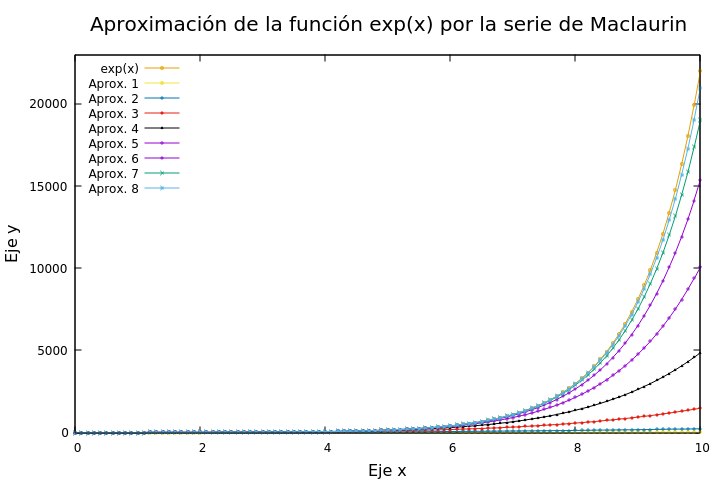
\includegraphics[width=12cm]{Maclaurinserie.png}
\caption{Aproximación de exp(x) usando la serie de Maclaurin}\label{fig:figura1}
\end{figure}
\begin{verbatim}
program taylor

    implicit none                  
        real (kind =8)::x,e_tay, re_taylor,exp_true
    integer::n,n1,t,j,k,npts
    npts=100
    t=15
    !Open file
   open (1,file="exp_taylor.txt",status="unknown") 
   !loop aproximation
   do k=1,t,2
      n1=k
   !loop terms
   do j=0,npts
    !Giving values to x
    x=0.1*real(j)
     !procesing the real functions
    exp_true= exp(x)
      ! call subroutine
    call exptaylor(x,n1,e_tay)
    re_taylor=e_tay
    !printing the results
    write(1,*) x, exp_true, re_taylor 
 end do
 write (1,*) " "
 write (1,*) " "
 end do
 close(1)

end program taylor

!==========================
subroutine exptaylor(x,n,exptay)
!==========================
    implicit none
    ! function arguments:
    integer :: i
    integer, intent(in):: n
    real (kind=8)::term,partial_sum
    real (kind=8), intent(in)::x
    real (kind=8),intent(out):: exptay
    
    !inicializando variables
    term = 1.
    partial_sum= term
    !Loop aproximations
    do i=1,n
        ! j'th term is  x**i / i!  which is the previous term times x/i:
        term = term*x/real(i)   
        ! add this term to the partial sum:
        partial_sum = partial_sum + term   
        end do
     exptay = partial_sum  ! this is the value returned
end subroutine exptaylor
\end{verbatim}
\section{Aproximación de la función sin(x)}
El código Fortran modificado para calcular la función sin(x), bajo las aproximaciones f1,f2,...,f10, usando la serie de Maclaurin segun muestra la gráfica 2, corresponde a:
\begin{figure}[htbp]
\centering
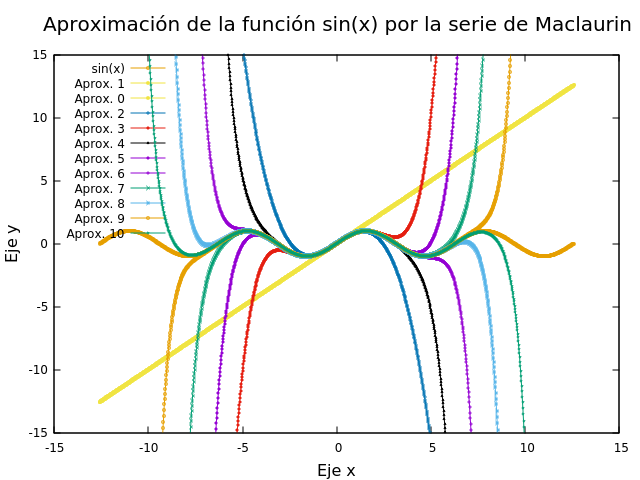
\includegraphics[width=12cm]{exp_sinx2.png}
\caption{Aproximación de sin(x) usando la serie de Maclaurin}\label{fig:figura2}
\end{figure}
\begin{verbatim}
program s_taylor
  !::::::::::::::::::::::::::::::::::::::::::::::::::::::::::::::::::::::
  ! APLICACIÓN FORTRAN PARA CALCULAR LA APROXIMACIÓN DE LA FUNCION Sin(x)
  ! USANDO LA SERIE DE MACLAURIN
  !sin_true---------------Función real de Sin(x)
  !y----------------------Aproximación 0 de sin(x)
  !x----------------------ángulos en radianes
  !stay-------------------Función Sin(x) aproximada
  !re_taylor--------------Función aproximada en la subrutina
  !:::::::::::::::::::::::::::::::::::::::::::::::::::::::::::::::::::::
    implicit none                  
    integer::n1,n,j,k,np,t
    real (kind=8), parameter:: pi=3.141592
    real (kind=8)::stay, re_taylor,x,sin_true,y
   
    !data in degrees
    np=720
    t=10
    do k=0,t

       n1=k
    !Open file
   open (1,file="sin_taylor.txt",status="unknown") 
  
        !loop terms
   do j=-np,np 
    !Giving values to x
      x=(pi*j)/180.
     !procesing the real functions
      sin_true= sin(x)
      y=x
      ! call subroutine
    call sintaylor(x,n1,stay)
    re_taylor=stay
    !printing the results
    write(1,*) x, sin_true, re_taylor,y
    end do
 write (1,*) " "
 write (1,*) " "
end do 
 close(1)
 
end program s_taylor

!::::::::::::::::::::::::::::::::::::::::::::::::::::::::::::::::
subroutine sintaylor(x,n,staylor
!:::::::::::::::::::::::::::::::::::::::::::::::::::::::::::::::
    implicit none
    ! function arguments:
    integer :: i
    integer, intent(in):: n
    real (kind=8)::term,partial_sum
    real (kind=8), intent(in)::x
    real (kind=8),intent(out):: staylor
    
  
    !inicializando variables
    term = x
    partial_sum= term
    !Loop aproximations
    do i=1,n
        ! j'th term is  x**i / i!  which is the previous term times x/i:
        term =(-1**i)*(term*x*x)/(2*i*(2*i+1))  
        ! add this term to the partial sum:
        partial_sum = partial_sum + term   
        end do
     staylor = partial_sum ! this is the value returned
end subroutine sintaylor
\end{verbatim}
\section{Observación}
La aproximación de la función sin(x), bajo las aproximaciones impares f1,f3,...,f15, produce la siguiente gráfica:
\begin{figure}[htbp]
\centering
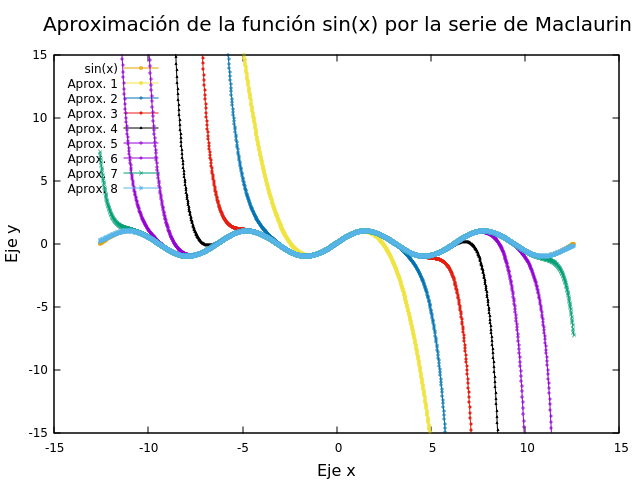
\includegraphics[width=12cm]{exp_sinx.png}
\caption{Aproximación de sin(x) usando la serie de Maclaurin, usando aproximaciones impares}\label{fig:figura3}
\end{figure}
\end{document}